\section{A morphism into the slaloms}\label{sec:construction}

We construct a morphism from $\mathfrak B;\mathfrak R$ to
$\mathfrak S_r$ for a suitable sequence $r$. This will give
$\nonM\leq\max\{\mathfrak b,\rr\}$.

\begin{lemma}\label{lem:morphism}
There is a function $r:\omega\to\omega\setminus\{0\}$ with
$r(n)\to\infty$ and a morphism
\[
 (\phi_-,\phi_+):\mathfrak B;\mathfrak R\longrightarrow\mathfrak S_r.
\]
\end{lemma}

\begin{proof}
Put $r(n)=8(2^{n+1})^4$ for $n<\omega$.
We shall define:
\[
\begin{aligned}
 \phi_-&:\omega^\omega\longrightarrow
              \omega^\omega\times{}^{\omega^\omega}\CC,\\
 \phi_+&:\omega^\omega\times\Sym\longrightarrow\mathcal S_r.
\end{aligned}
\]

For each $g\in\omega^\omega$ and $n\in \omega$ with $g(n)>0$, apply Lemma~\ref{lem:finite}
with $m=g(n)$ and $q=2^{n+1}$ to obtain a positive integer $L_n^g$ and
balanced vectors $(v_{n,k}^g)_{k<g(n)}$ in $\{-1/L_n^g,1/L_n^g\}^{L_n^g}$
such that, for every $\sigma\in\operatorname{Sym}(L_n^g)$,
\begin{equation}\label{eq:finite-block-bound}
 \left|\{k<g(n):M_\sigma(v_{n,k}^g)>1/2^{n+1}\}\right|
 \leq 4(2^{n+1})^4=\frac{r(n)}2.
\end{equation}
If $g(n)=0$, put $L_n^g=1$.

Partition $\omega$ into successive intervals $(I_n^g:n<\omega)$
of lengths $L_n^g$. For $k<g(n)$, define $u_{n,k}^g$ by placing $v_{n,k}^g$ on $I_n^g$:
\[
 u_{n,k}^g(i)=
 \begin{cases}
  v_{n,k}^g(i-\min I_n^g),&i\in I_n^g,\\
  0,&i\notin I_n^g.
 \end{cases}
\]
Thus $u_{n,k}^g$ is supported on $I_n^g$, with sum zero and absolute
sum one.

\begin{figure}[htbp]
\centering
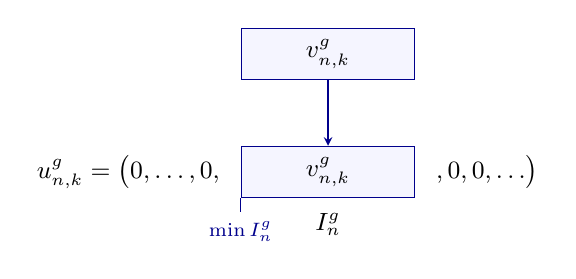
\begin{tikzpicture}[font=\small, >=stealth,
 block/.style={draw=blue!55!black,fill=blue!4,
 minimum width=2.2cm,minimum height=0.65cm}]
 \node[block] (v) at (0,1.5) {$v_{n,k}^g$};
 \node[block] (u) at (0,0) {$v_{n,k}^g$};
 \draw[->,blue!55!black] (v.south) -- (u.north);
 \node[anchor=east] at (-1.25,0) {$u_{n,k}^g=\bigl(0,\ldots,0,$};
 \node[anchor=west] at (1.25,0) {$,0,0,\ldots\bigr)$};
 \node[below] at (0,-0.4) {$I_n^g$};
 \draw[blue!55!black] (u.south west) -- ++(0,-0.18)
  node[below,font=\scriptsize] {$\min I_n^g$};
\end{tikzpicture}
\caption{Placing $v_{n,k}^g$ on $I_n^g$ and extending by zero.}
\label{fig:block-embedding}
\end{figure}

For $\pi\in\Sym$, define the response map by
\begin{equation}\label{eq:bad-slalom}
 \phi_+(g,\pi)(n)=
 \{k<g(n):M(u_{n,k}^g)>1/2^{n+1}
                  \text{ or }M_\pi(u_{n,k}^g)>1/2^{n+1}\}.
\end{equation}

\begin{claim}
For every $g\in\omega^\omega$ and $\pi\in\Sym$, the sequence
$\phi_+(g,\pi)$ is an $r$-slalom.
\end{claim}

\begin{proof}[Proof of the claim]
Fix $n<\omega$. If $g(n)=0$, then $\phi_+(g,\pi)(n)=\varnothing$,
so the required bound is immediate. Assume $g(n)>0$.
Let $\pi_n^{g}\in\operatorname{Sym}(L_n^g)$ list the coordinates of
$I_n^g$ in the order in which $\pi$ visits them. Write
\[
    \pi^{-1}[I_n^g]=\{t_0<\cdots<t_{L_n^g-1}\}
\]
and define
\[
    \pi_n^g(i)=\pi(t_i)-\min I_n^g\qquad(i<L_n^g).
\]
Thus, the mapping
$s\mapsto\pi^{-1}(\min I_n^g+\pi_n^{g}(s))$ from $L_{n}^g$ to $\pi^{-1}[I_n^g]$ is a strictly increasing bijection.
For this reason, for every $k<g(n)$ and $j<\omega$,
\[
 S_j^\pi(u_{n,k}^g)=S_{|\pi[j]\cap I_n^g|}^{\pi_n^{g}}(v_{n,k}^g),
\]
and therefore $M_\pi(u_{n,k}^g)=M_{\pi_n^{g}}(v_{n,k}^g)$.
Thus, by \eqref{eq:finite-block-bound},
\[
    |\{k<g(n):M_{\pi_n^{g}}(v_{n,k}^g)>1/2^{n+1}\}|
    \leq 4(2^{n+1})^4=\frac{r(n)}2.
\]
Similarly, $M(u_{n,k}^g)=M(v_{n,k}^g)$, so the same
estimate applies to the first condition in \eqref{eq:bad-slalom}. Hence
\begin{equation*}
 |\phi_+(g,\pi)(n)|\leq\frac{r(n)}2+\frac{r(n)}2=r(n).
\end{equation*}
\end{proof}

Next, for $e\in\omega^\omega$, let $A_e^g=\{n<\omega:e(n)<g(n)\}$ and define, coordinatewise,
\begin{equation*}
 a_e^g=\sum_{n\in A_e^g}u_{n,e(n)}^g.
\end{equation*}
Notice that each $i<\omega$ belongs to
a unique interval $I_n^g$, and every summand supported on another
interval vanishes at $i$. Thus, for this $n$, which depends on $i$, we have
\[
 a_e^g(i)=
 \begin{cases}
  u_{n,e(n)}^g(i),&n\in A_e^g,\\
  0,&n\notin A_e^g,
 \end{cases}
 \qquad\text{where }i\in I_n^g.
\]
In particular, $a_e^g$ is well-defined.

\begin{claim}
If $e<^\infty g$ and $e\notin^\infty\phi_+(g,\pi)$, then
$a_e^g\in\CC$ and both its natural sum and its $\pi$-rearranged sum
are zero.
\end{claim}

\begin{proof}[Proof of the claim]
Since $e<^\infty g$, the set $A_e^g$ is infinite, so
\begin{equation}\label{eq:absolute}
 \sum_{i\in \omega}|a_e^g(i)|
 =\sum_{n\in A_e^g}\sum_{i\in I_n^g}|u_{n,e(n)}^g(i)|
 =\sum_{n\in A_e^g}1=\infty.
\end{equation}
Fix $\rho\in\{\operatorname{id}_\omega,\pi\}$ and $\eta>0$.
Choose $N$ such that $2^{-N}<\eta$ and
$e(n)\notin\phi_+(g,\pi)(n)$ for every $n\geq N$.
For $n\in A_e^g$ with $n\geq N$, \eqref{eq:bad-slalom} gives
$M_\rho(u_{n,e(n)}^g)\leq1/2^{n+1}$.
For each $j$, the finite set $\rho[j]$ meets only finitely many of
the disjoint intervals $I_n^g$. Grouping the terms of the partial sum
according to these intervals gives
\[
\begin{aligned}
 S_j^\rho(a_e^g)
 &=\sum_{i\in\rho[j]}a_e^g(i)\\
 &=\sum_{n\in A_e^g}\sum_{i\in\rho[j]\cap I_n^g}u_{n,e(n)}^g(i)
 =\sum_{n\in A_e^g}S_j^\rho(u_{n,e(n)}^g).
\end{aligned}
\]
Only finitely many summands in the outer sums are nonzero.

Since $\bigcup_{n<N}I_n^g$ is finite, choose $J$ such that
$\bigcup_{n<N}I_n^g\subseteq\rho[J]$.
For every $j\geq J$ and $n\in A_e^g$ with $n<N$,
$S_j^\rho(u_{n,e(n)}^g)=\sum_{i\in I_n^g}u_{n,e(n)}^g(i)=0$.


Thus, for $j\geq J$ we have
\[
\begin{aligned}
 |S_j^\rho(a_e^g)|
 &=\left|\sum_{\substack{n\in A_e^g\\n\geq N}}
                  S_j^\rho(u_{n,e(n)}^g)\right|\\
 &\leq\sum_{\substack{n\in A_e^g\\n\geq N}}
                   |S_j^\rho(u_{n,e(n)}^g)|\\
 &\leq\sum_{\substack{n\in A_e^g\\n\geq N}}M_\rho(u_{n,e(n)}^g)\\
 &\leq\sum_{n\geq N}\frac1{2^{n+1}}=2^{-N}<\eta.
\end{aligned}
\]
Since $\eta>0$ was arbitrary, $S_j^\rho(a_e^g)\to0$.
Taking $\rho=\operatorname{id}_\omega$ and $\rho=\pi$ gives the two
asserted sums, and \eqref{eq:absolute} gives conditional convergence.
\end{proof}

To define the challenge map, fix any $a^*\in\CC$ and put
\[
 \phi_-(e)=(e,f_e),\qquad
 f_e(g)=
 \begin{cases}
  a_e^g,&a_e^g\in\CC,\\
  a^*,&\text{otherwise}.
 \end{cases}
\]
Finally, suppose $(g,\pi)$ responds to $\phi_-(e)$. This means
$e<^\infty g$ and $\pi$ rearranges $f_e(g)$.
If $e\notin^\infty\phi_+(g,\pi)$, the preceding claim gives
$a_e^g\in\CC$ and shows that $\pi$ preserves its sum.
But then $f_e(g)=a_e^g$, a contradiction.
Therefore $e\in^\infty\phi_+(g,\pi)$, verifying the morphism condition.
\end{proof}

Consequently, Theorem~\ref{thm:main} holds.
\begin{proof}[Proof of Theorem~\ref{thm:main}]
By Lemma~\ref{lem:morphism}, there exists $r:\omega\to\omega\setminus\{0\}$ with $r(n)\to\infty$ and a morphism
\[
 (\phi_-,\phi_+):\mathfrak B;\mathfrak R\longrightarrow\mathfrak S_r.
\]
By Remark~\ref{rem:sequential-norm} and the known bound
$\mathfrak b\leq\rr$ from Theorem~\ref{thm:known-sandwich},
\[
\begin{aligned}
 \nonM=\|\mathfrak S_r\|
 &\leq\|\mathfrak B;\mathfrak R\|\\
 &=\max\{\|\mathfrak B\|,\|\mathfrak R\|\}
 =\max\{\mathfrak b,\rr\}=\rr.
\end{aligned}
\]
The reverse inequality $\rr\leq\nonM$ is also part of
Theorem~\ref{thm:known-sandwich}.
\end{proof}
